\documentclass[12pt]{article}

\usepackage{../thesis}

\usepackage{tikz} 

\begin{document}

\pagestyle{empty}

\begin{tikzpicture}
    \node[anchor=south west,inner sep=0] (image) at (0,0) {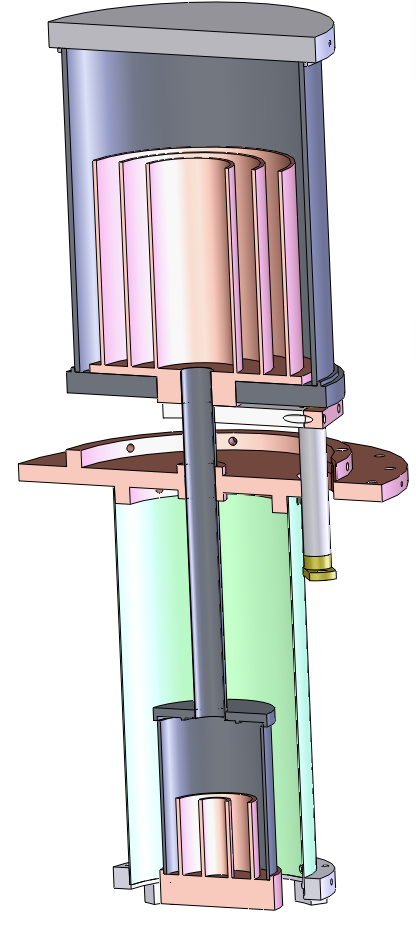
\includegraphics[width=2.7in]{../images/he4-sorp-fridge-cutaway.png}};
    \begin{scope}[x={(image.south east)},y={(image.north west)}]
	    %\draw[help lines,xstep=.1,ystep=.1] (0,0) grid (1.5,1);
		%\foreach \x in {0,1,...,15} { \node [anchor=north] at (\x/10,0) {0.\x}; }
		%\foreach \y in {0,1,...,9} { \node [anchor=east] at (0,\y/10) {0.\y}; }
        \draw[blue,ultra thick,rounded corners] (0.10,0.56) rectangle (0.86,1.01) node[below left] {\textbf{A}}; % pump
        \draw[blue,ultra thick,rounded corners] (0.02,0.56) rectangle (1.03,0.44) node[above left] {\textbf{B}}; % cond plate
        \draw[blue,ultra thick,rounded corners] (0.70,0.56) rectangle (0.88,0.36) node[above left] {\textbf{C}}; % heat switch
        \draw[blue,ultra thick,rounded corners] (0.35,0.25) rectangle (0.72,-0.02) node[above left] {\textbf{D}}; % pot
        
		\draw[thick,<->] (0.9,0.02) -- ++(0,0.21875) node[midway,right] {3 in}; % scale bar
    \end{scope}
\end{tikzpicture}

\end{document}
